\documentclass[final,hyperref={pdfpagelabels=false}]{beamer}
\mode<presentation>
  {
  %  \usetheme{Berlin}
  \usetheme{Dreuw}
  }
  \usepackage{times}
  \usepackage{amsmath,amsthm, amssymb, latexsym}
  \boldmath
  \usepackage[english]{babel}
  \usepackage[latin1]{inputenc}
  \usepackage[orientation=portrait,size=a0,scale=1.4,debug]{beamerposter}

  %%%%%%%%%%%%%%%%%%%%%%%%%%%%%%%%%%%%%%%%%%%%%%%%%%%%%%%%%%%%%%%%%%%%%%%%%%%%%%%%%5
  \graphicspath{{figures/}}
  \title[Projeto Orientado em Computação II]{Obstructed wireless networks with COOJA extended}
  \author[Manasses \& Olga]{Manasses Ferreira Neto}
  \institute[WISEMAP DCC UFMG]{Wireless Informational Sensing Embedded systems Models Algorithms and Protocols, Computer Science Department DCC, Minas Gerais Federal University}
  \date{Nov. 14th, 2014}


  %%%%%%%%%%%%%%%%%%%%%%%%%%%%%%%%%%%%%%%%%%%%%%%%%%%%%%%%%%%%%%%%%%%%%%%%%%%%%%%%%5
  \begin{document}
  \begin{frame}{} 
    \begin{columns}[t]
      \begin{column}{.48\linewidth}
        \begin{block}{Introduction}
          \centering
          The model is based on a grid structure of one-dimensional street segments and
          two-dimensional street intersections. This structure provides a realistic representation
          of a variety of network scenarios with obstacles and, at the same time, allows a simple
          enough analysis
          \newline
          About the use of the simulator COOJA extended throw a class made by the authors with 
          intents to study obstructed wireless networks
         
        \end{block}
      \end{column}
      \begin{column}{.48\linewidth}
        \begin{block}{Related Work}
          \begin{itemize}
          \item Model and Analytical CTR: [Almiron et al. 2013] 
          $$ r_{c} = \frac{ln(g)+ln(\mu-1)}{\mu}, \epsilon \geq \epsilon_{c}$$
          \item UDG Tractability Theory:[Clark et al. 1990]
          \item Aprox. Algorithm for Visibility Improvement: [Erlebach et al. 2005]
          \end{itemize}      
        \end{block}        
      \end{column}
    \end{columns}  
    \vfill
    \begin{block}{Results}
      \centering

      Due the long time spent it with the simulations, we are dedicating to distribute
      the computation using a simple server-client protocol routine made it from scratch by the
      authors.
      Furthermore, we will study forms to efficiently handles with the visibility calcu-
      lations. That are at this moment very expensive, mainly for the MRM model. At mo-
      ment, we are investigating the shifting-strategy with dynamic-programming described at
      [Erlebach et al. 2005]
      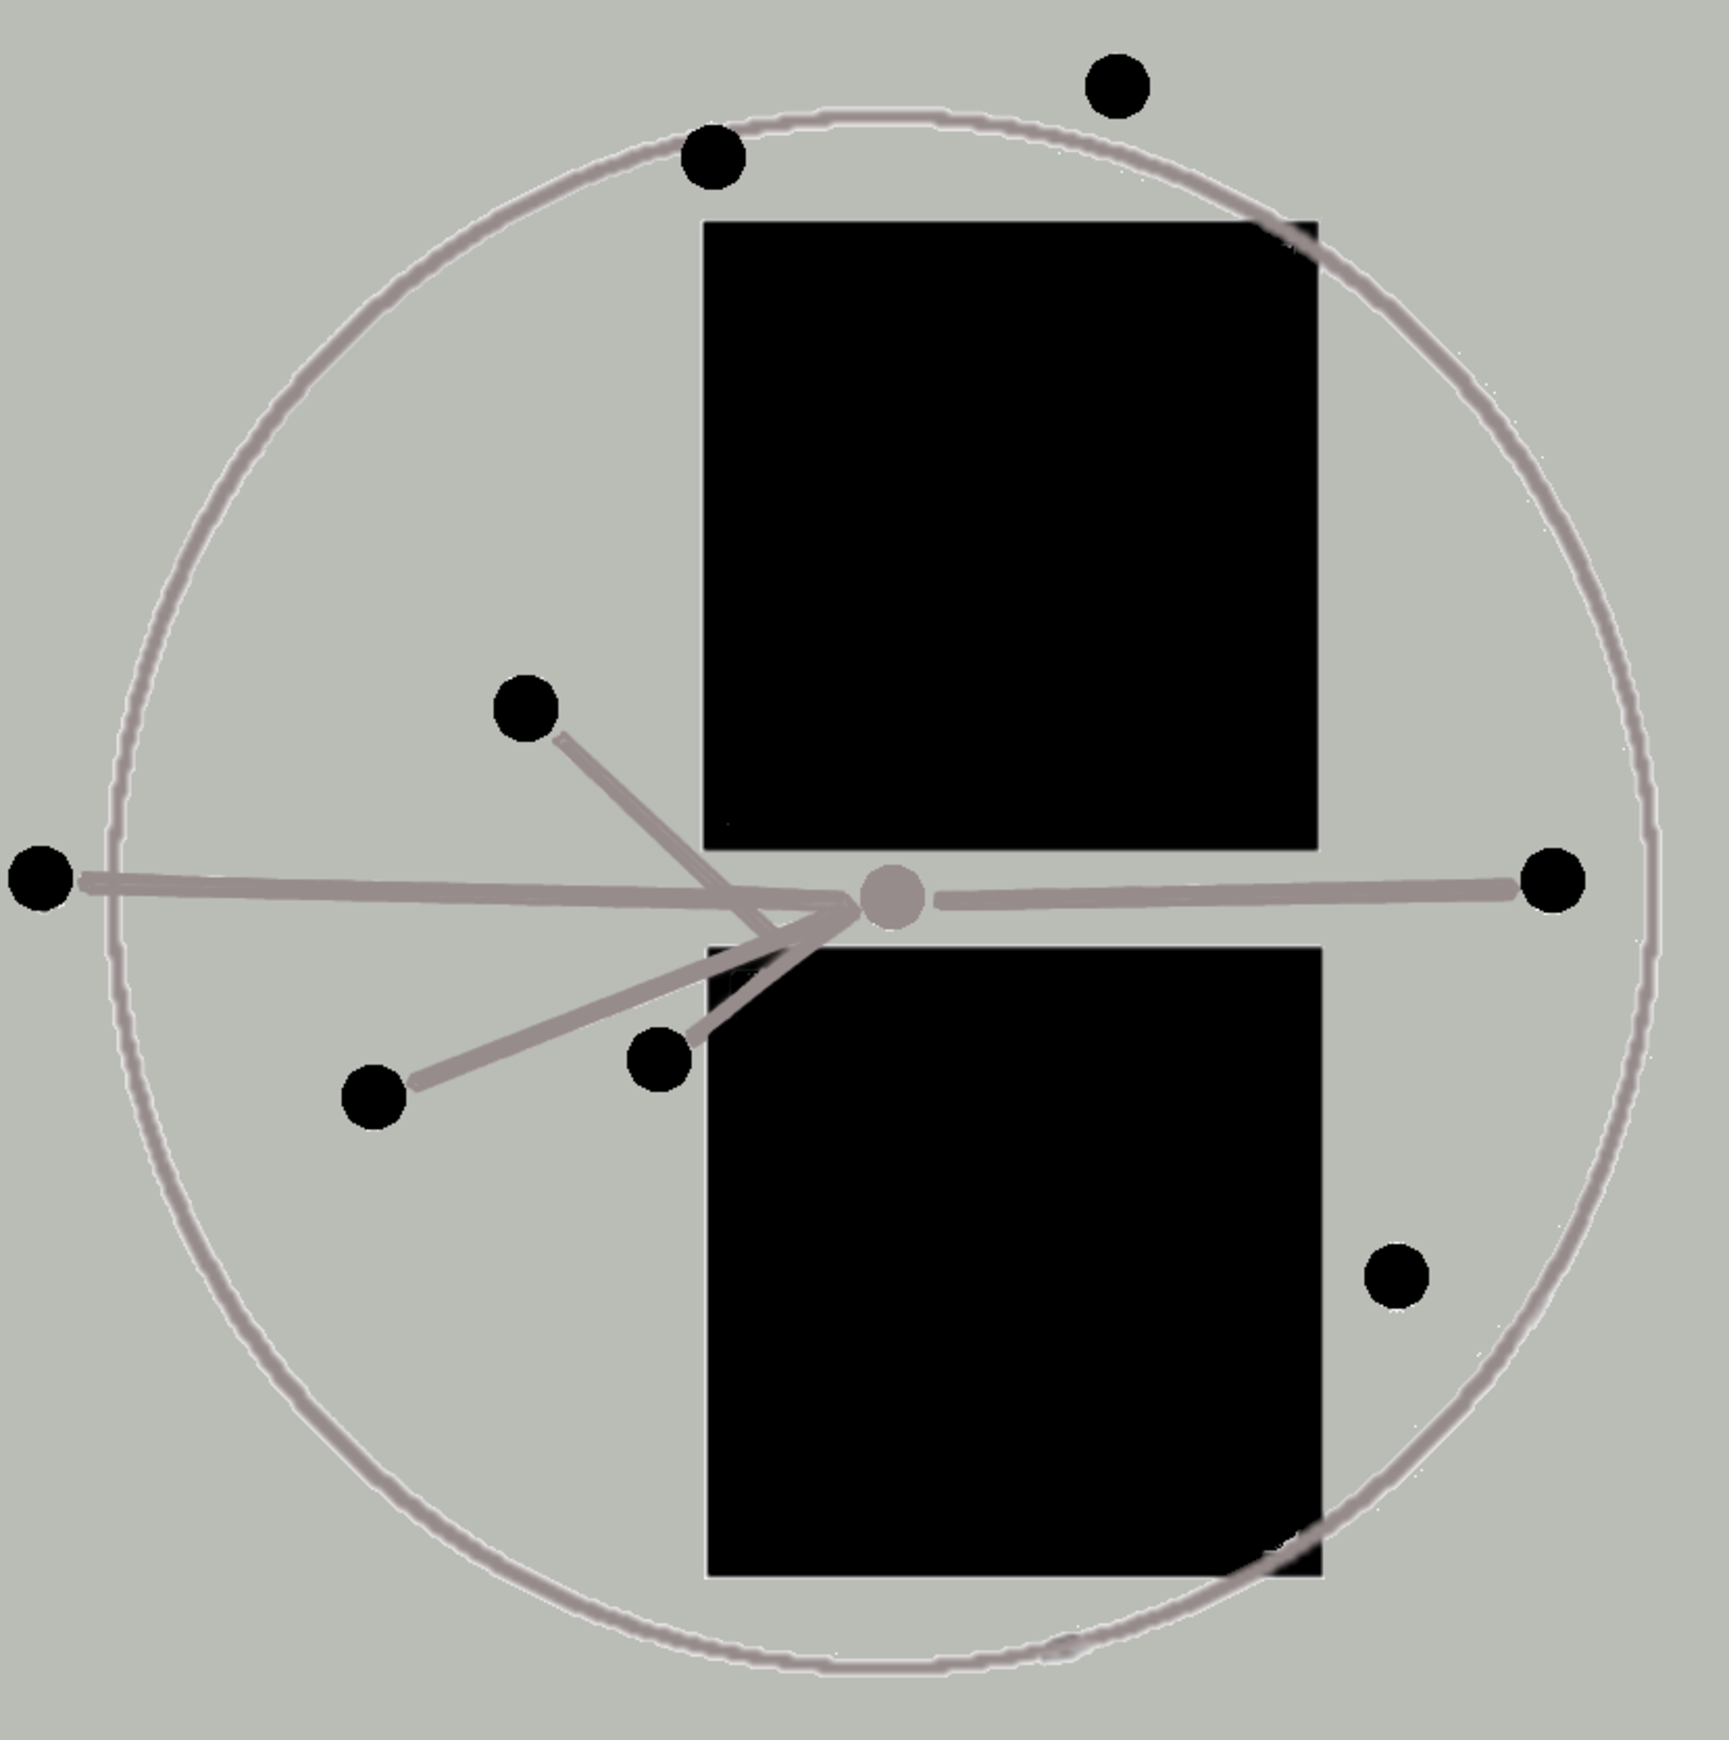
\includegraphics[width=0.20\linewidth]{udgo}          
      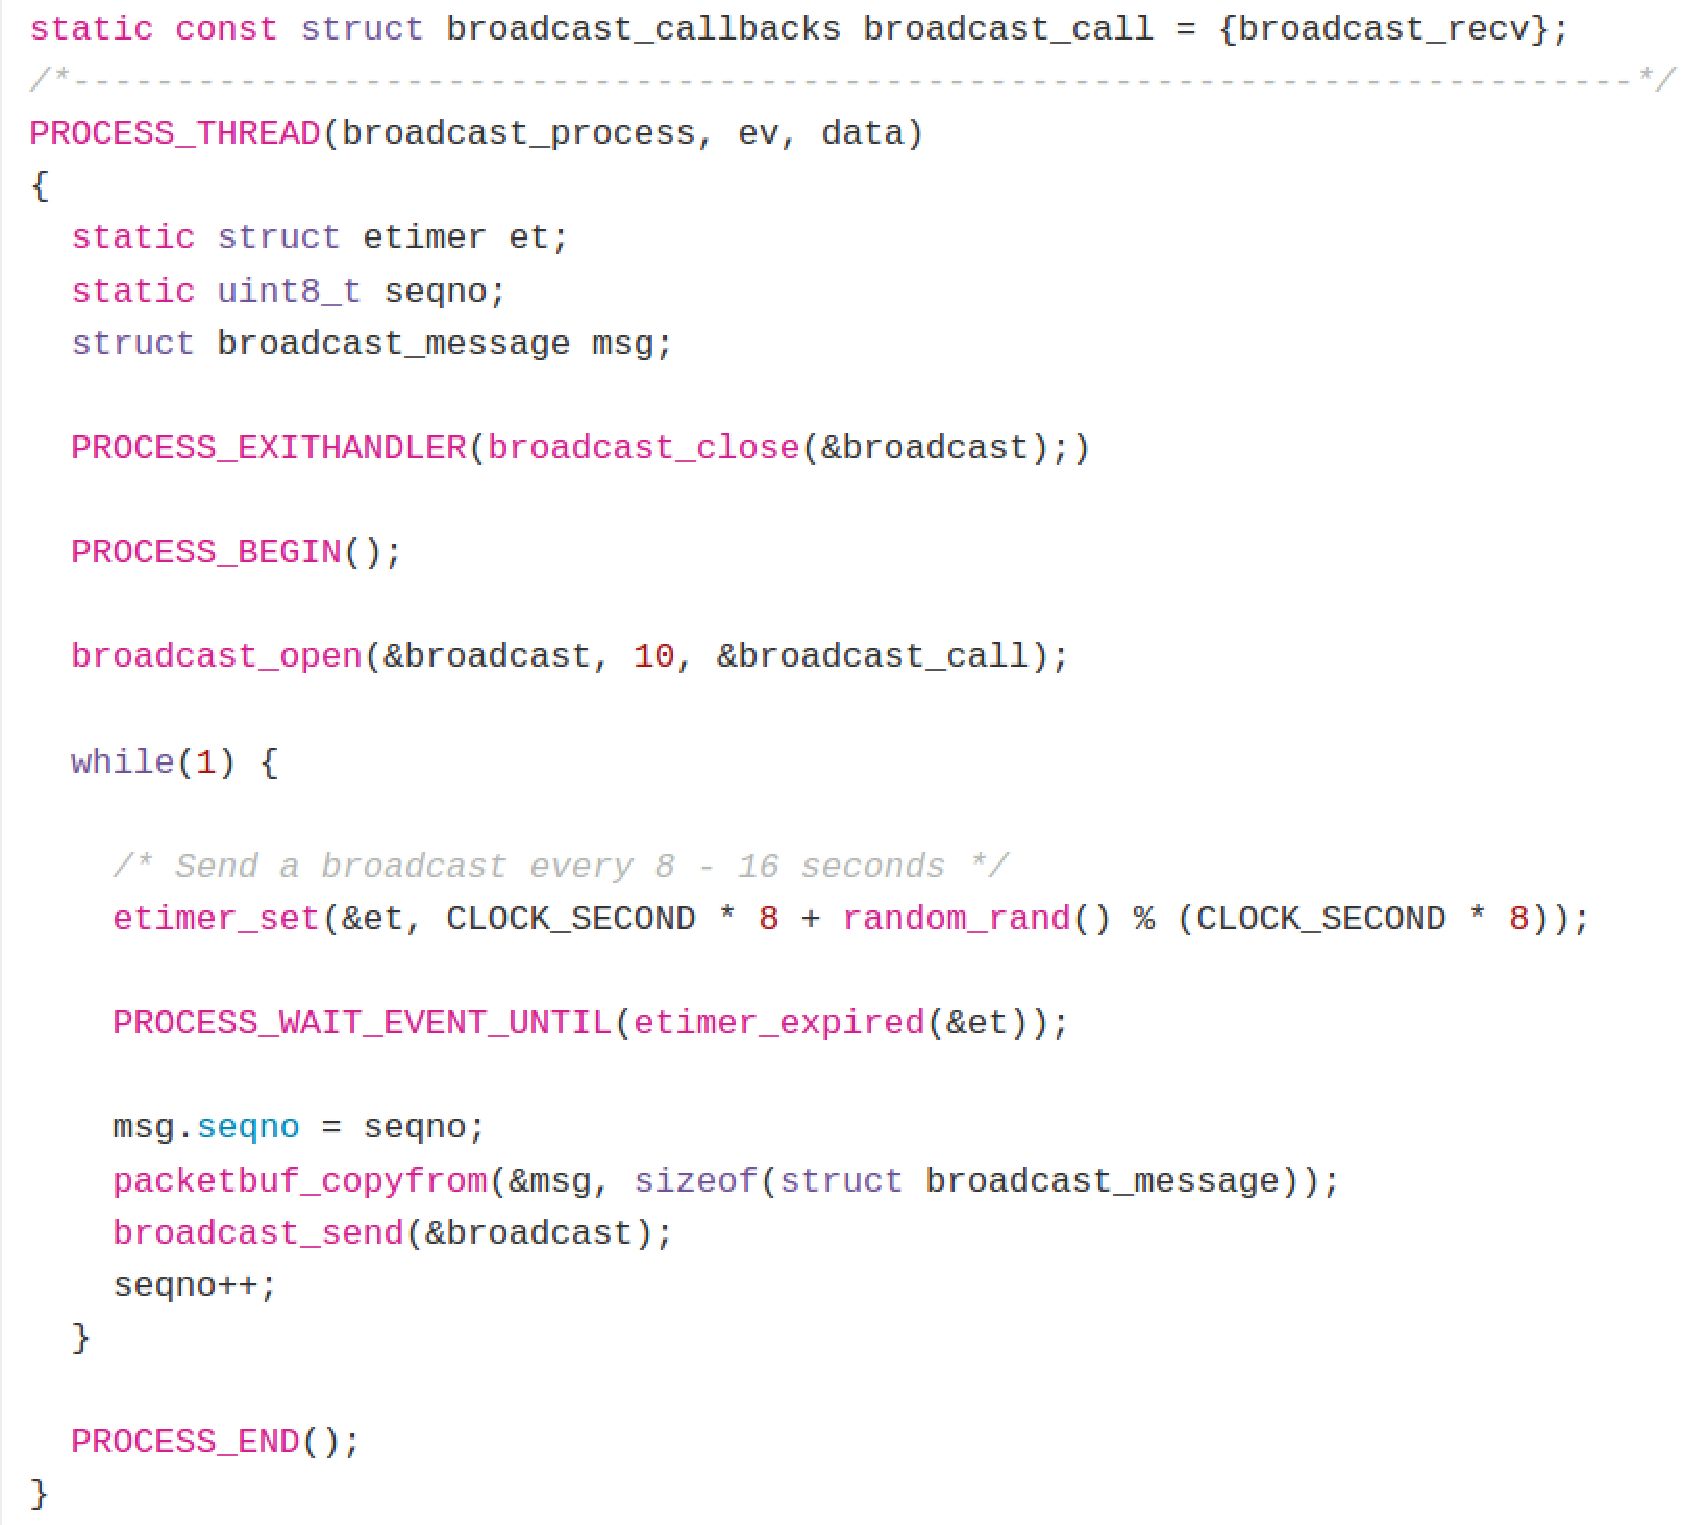
\includegraphics[width=0.20\linewidth]{node-code}
      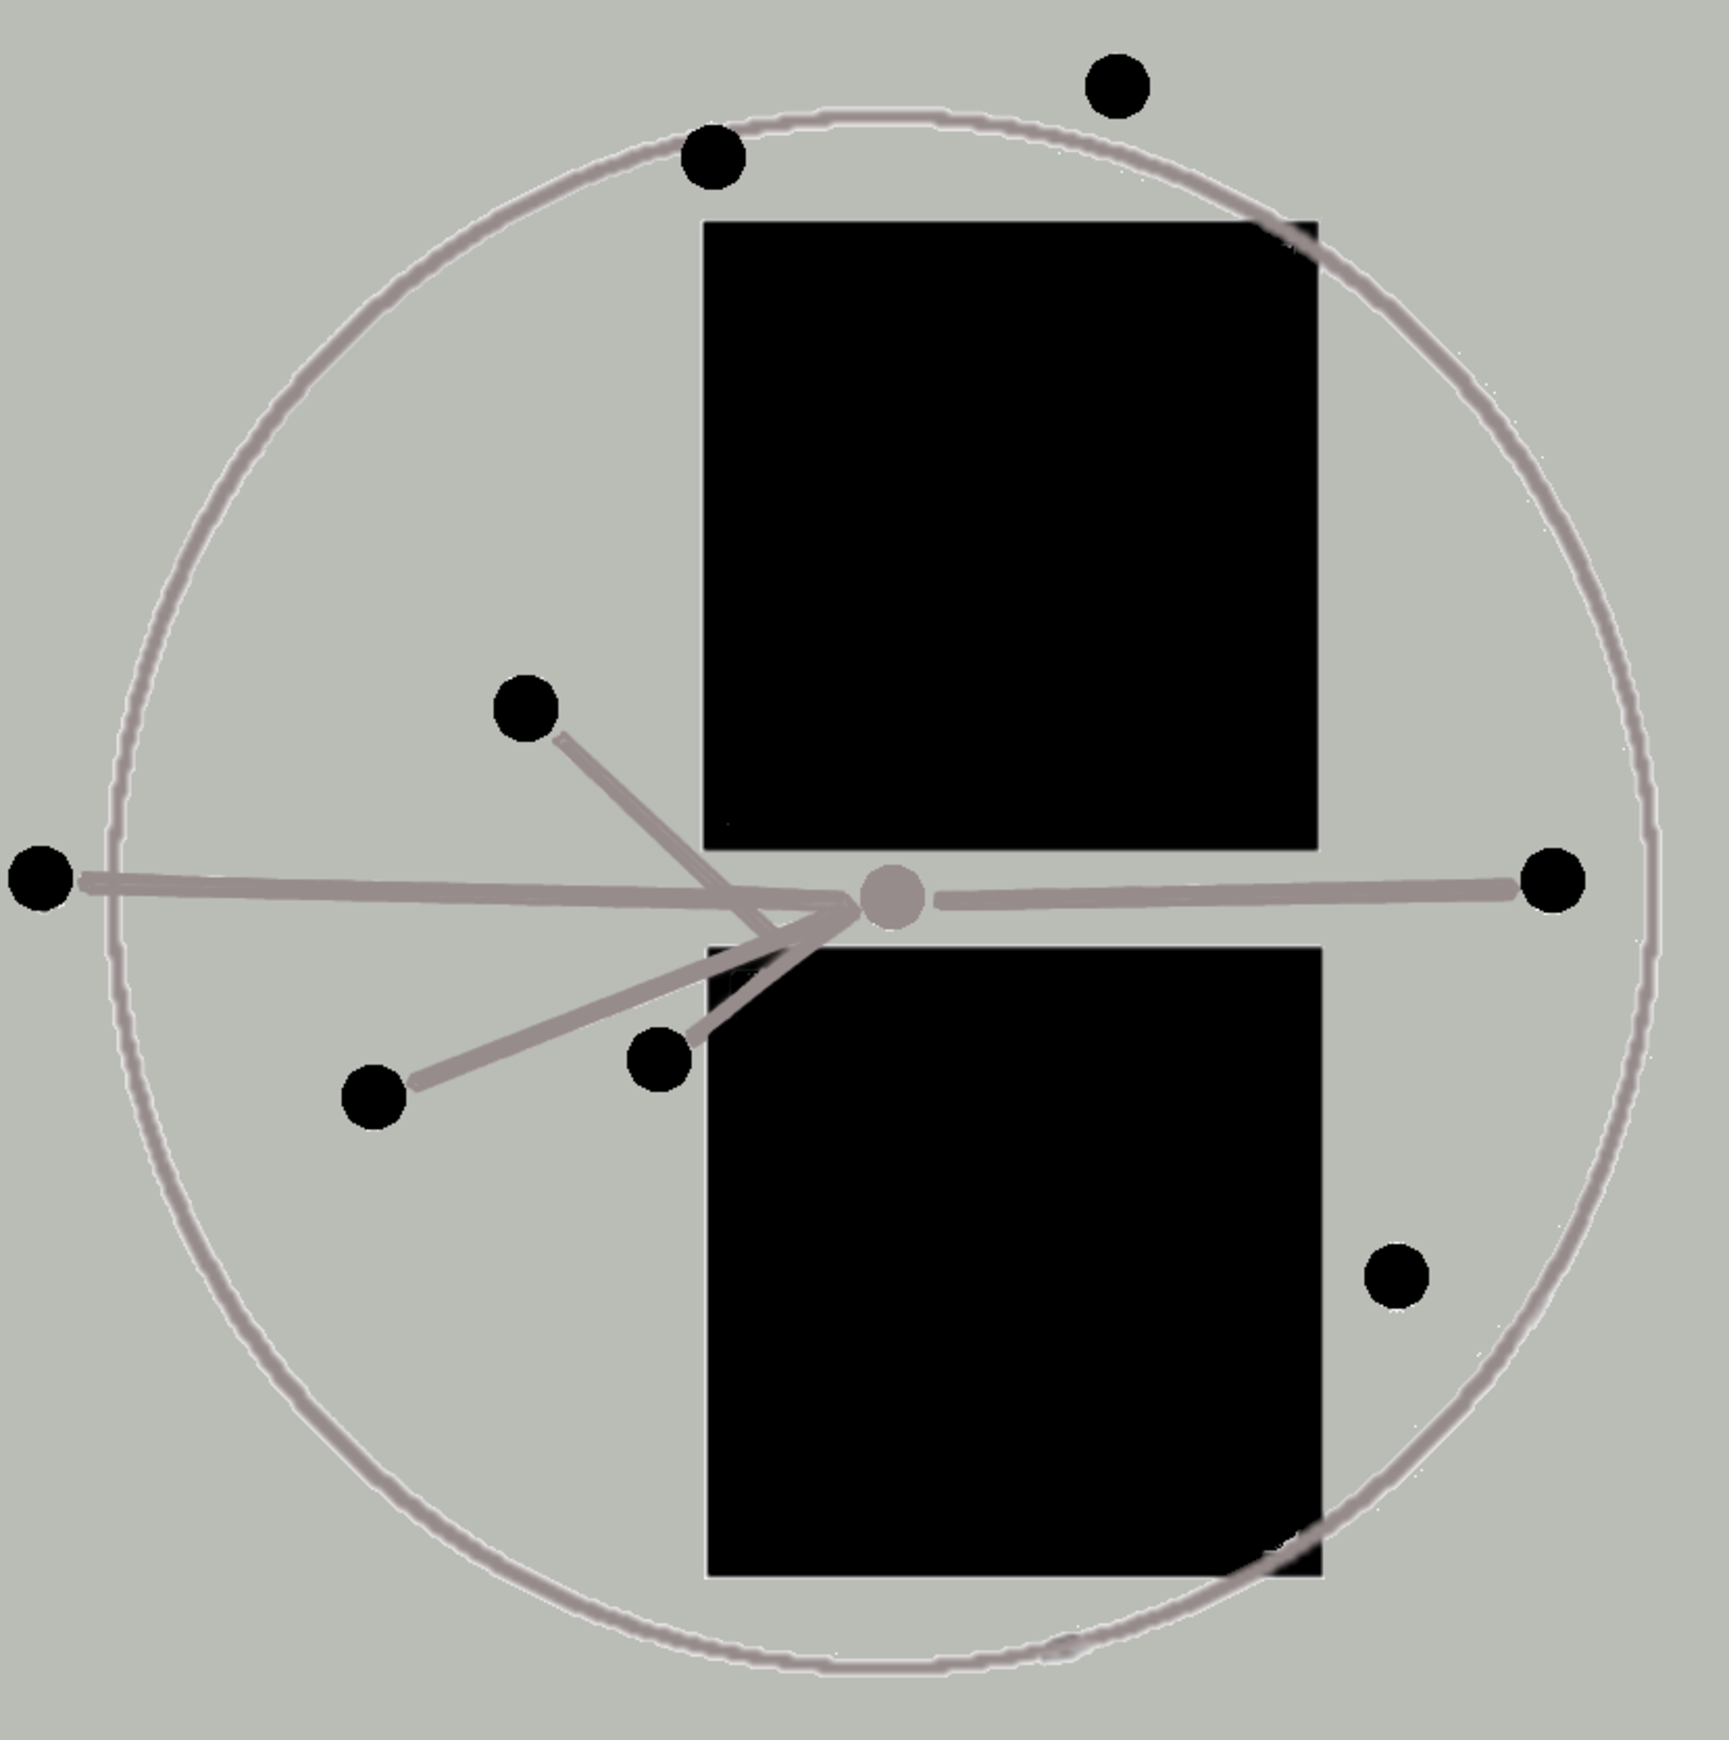
\includegraphics[width=0.20\linewidth]{udgo}          
      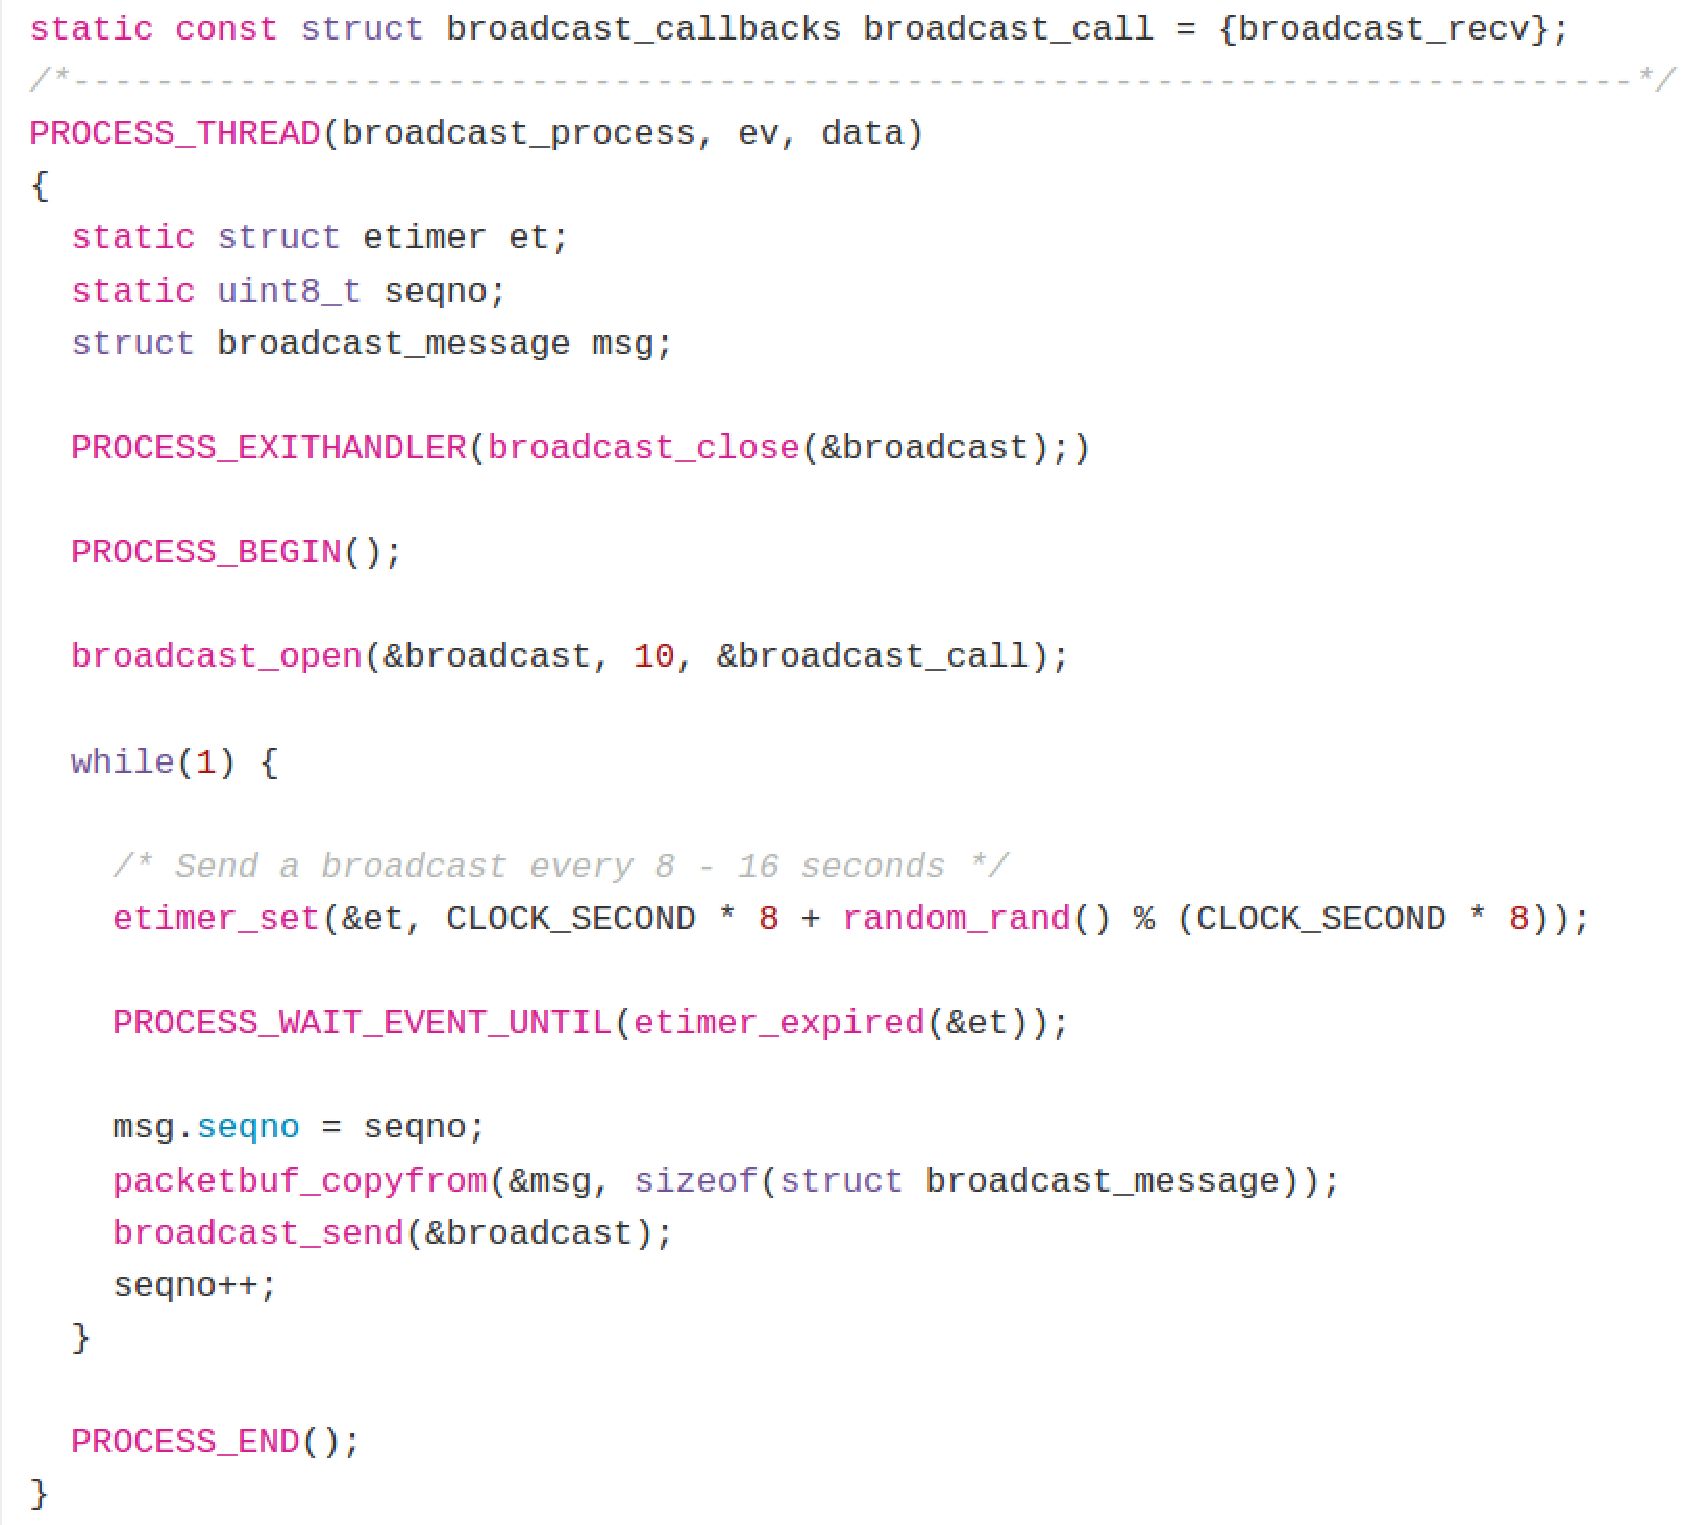
\includegraphics[width=0.20\linewidth]{node-code}      
      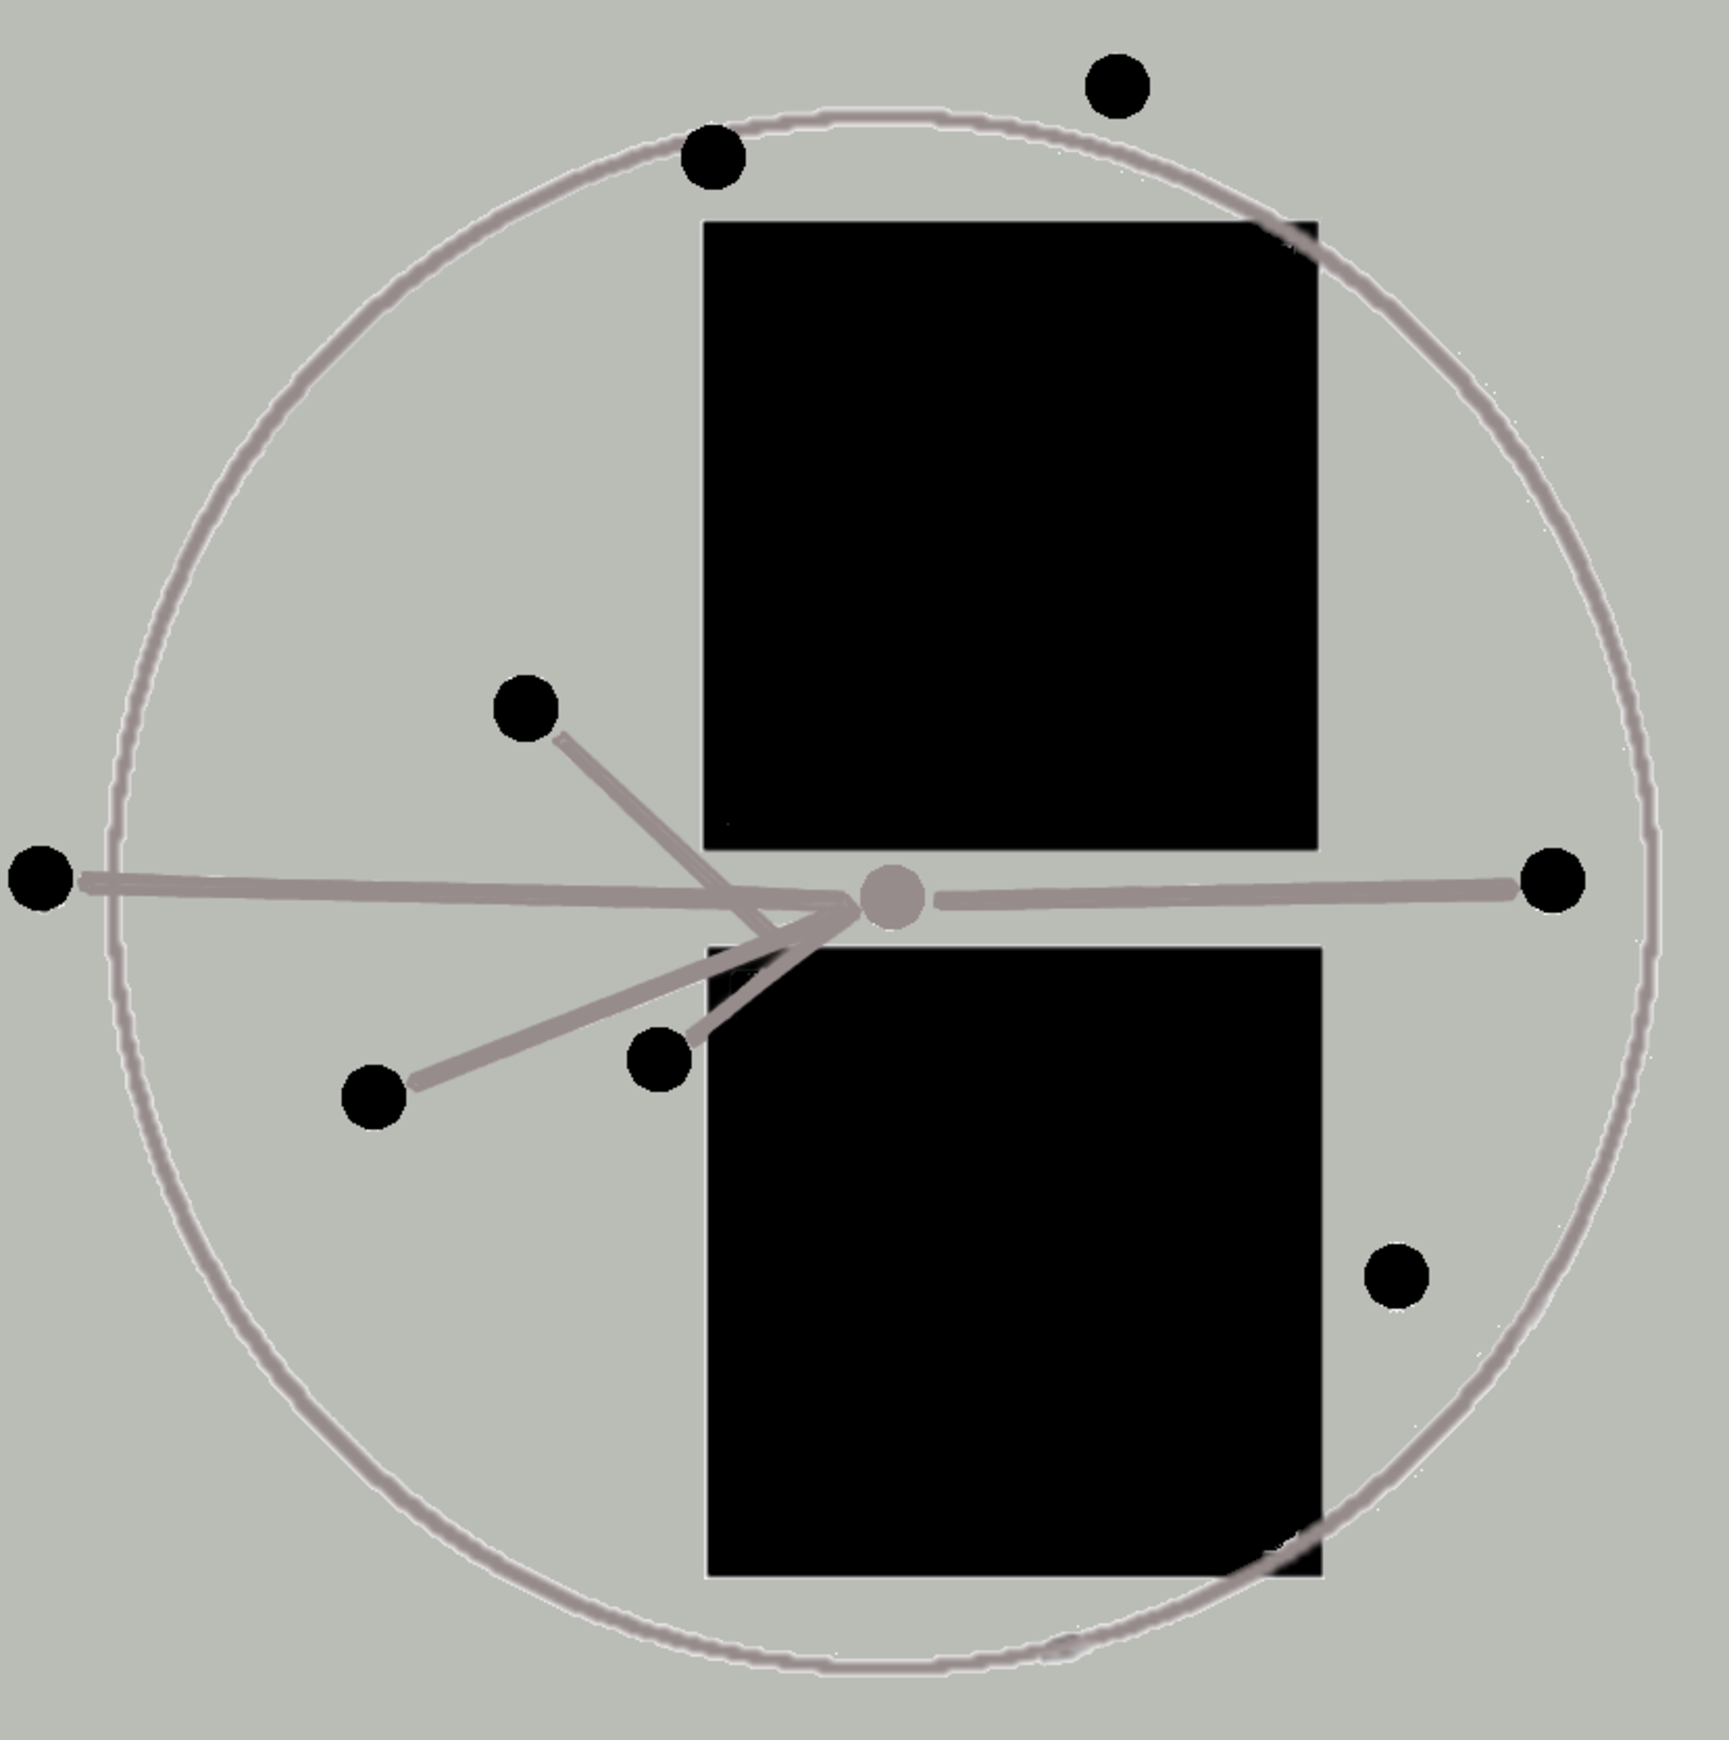
\includegraphics[width=0.20\linewidth]{udgo}          
    \end{block}
    \vfill
    \vfill
    \vfill
    \begin{columns}[t]
      \begin{column}{.48\linewidth}
        \begin{block}{\large Questions we made}
          \centering
            Analytical CTR will be greater than experimental? \newline
            Physical aspects of MRM could increase the visibility? \newline And the connectivity? \newline
            For the same properties, what the interference will cause? \newline
            How can we feedback model by the physical UDGO?
        \end{block}
        \begin{block}{POC1}
          \centering
          On the first part of this work, we implemented an abstract medium at
          COOJA named UDGO gathering two pre-existing models UDGM and MRM.
          [Osterlind et al. 2006]
          UDGM inserts the Unit Disk Graph behaviour, being more simple. MRM leads
          with the physical aspect of the transmission, being much more complex\newline
          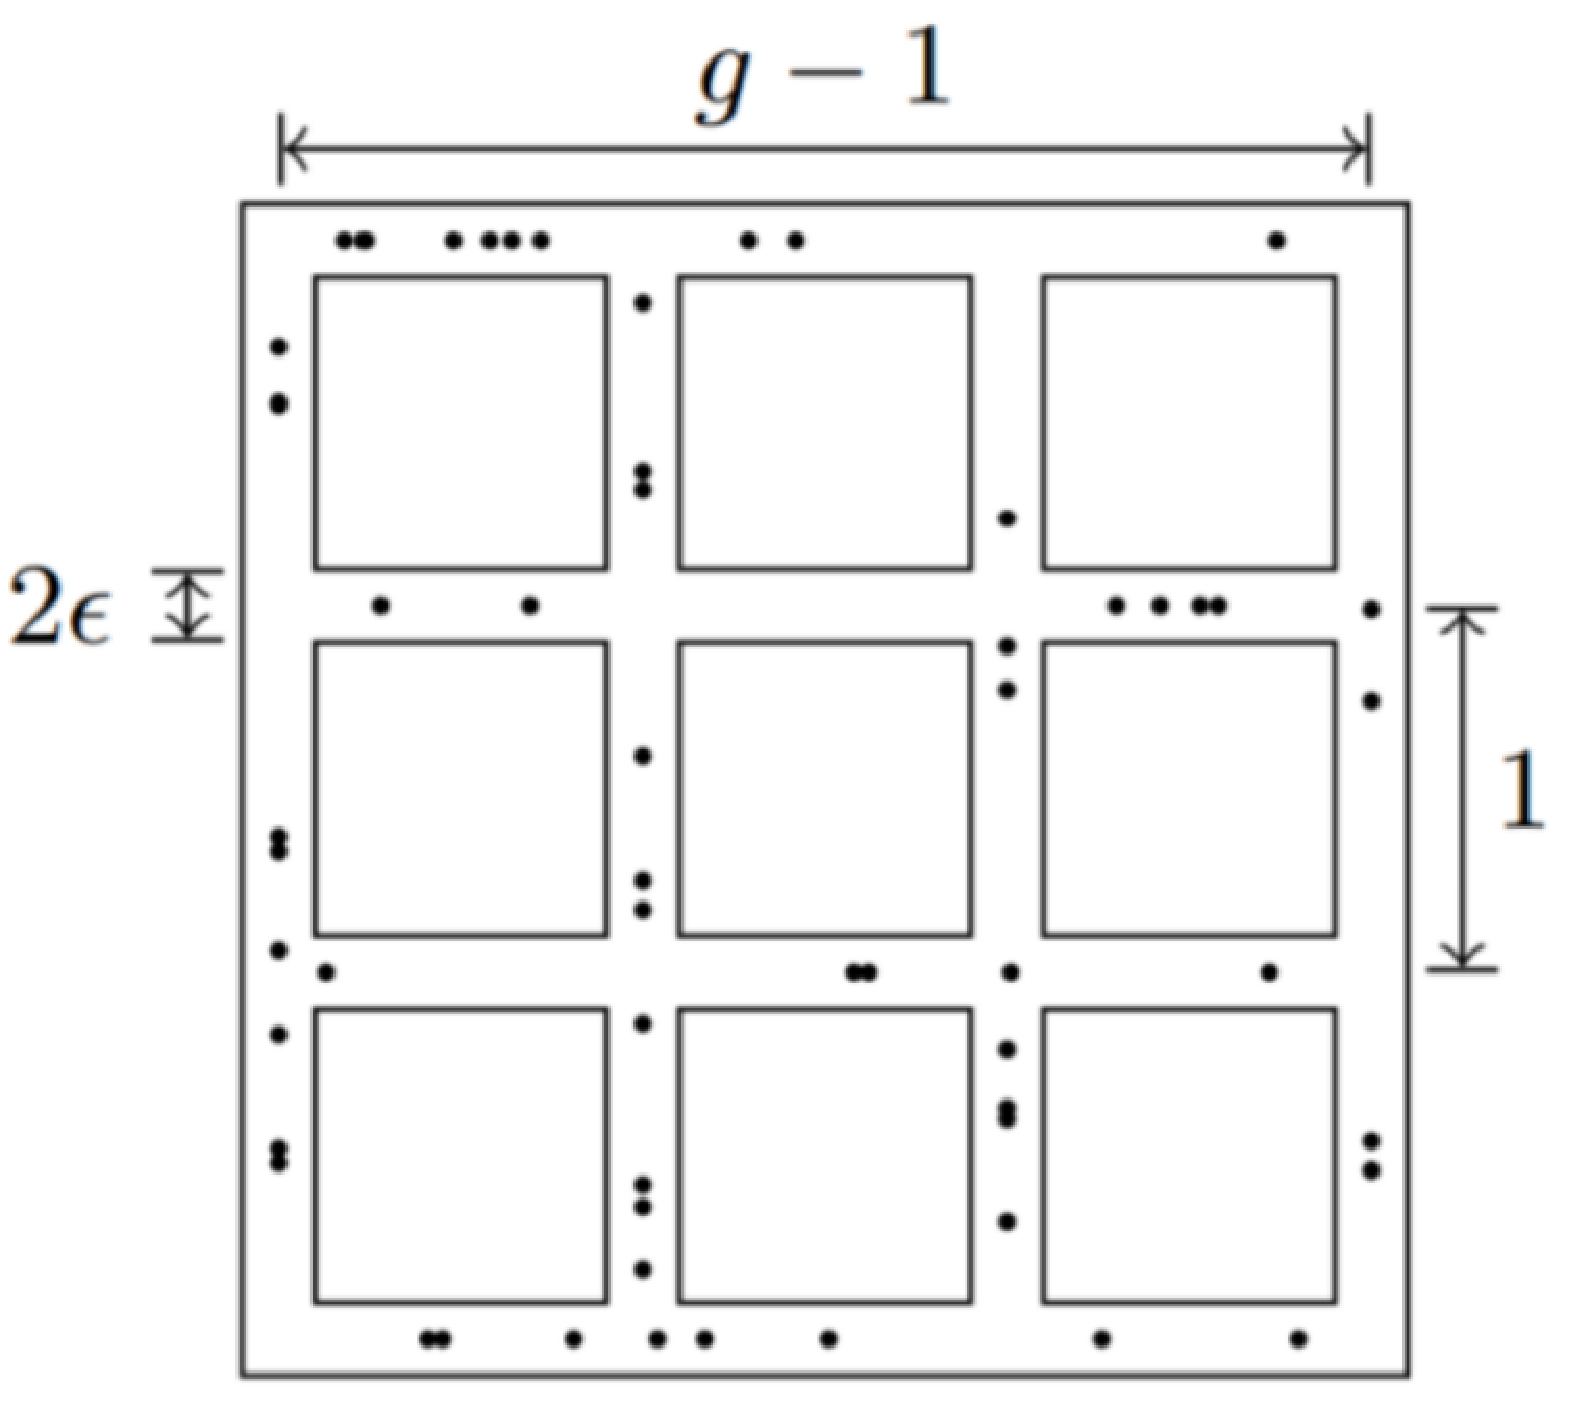
\includegraphics[width=0.3\linewidth]{grid}
          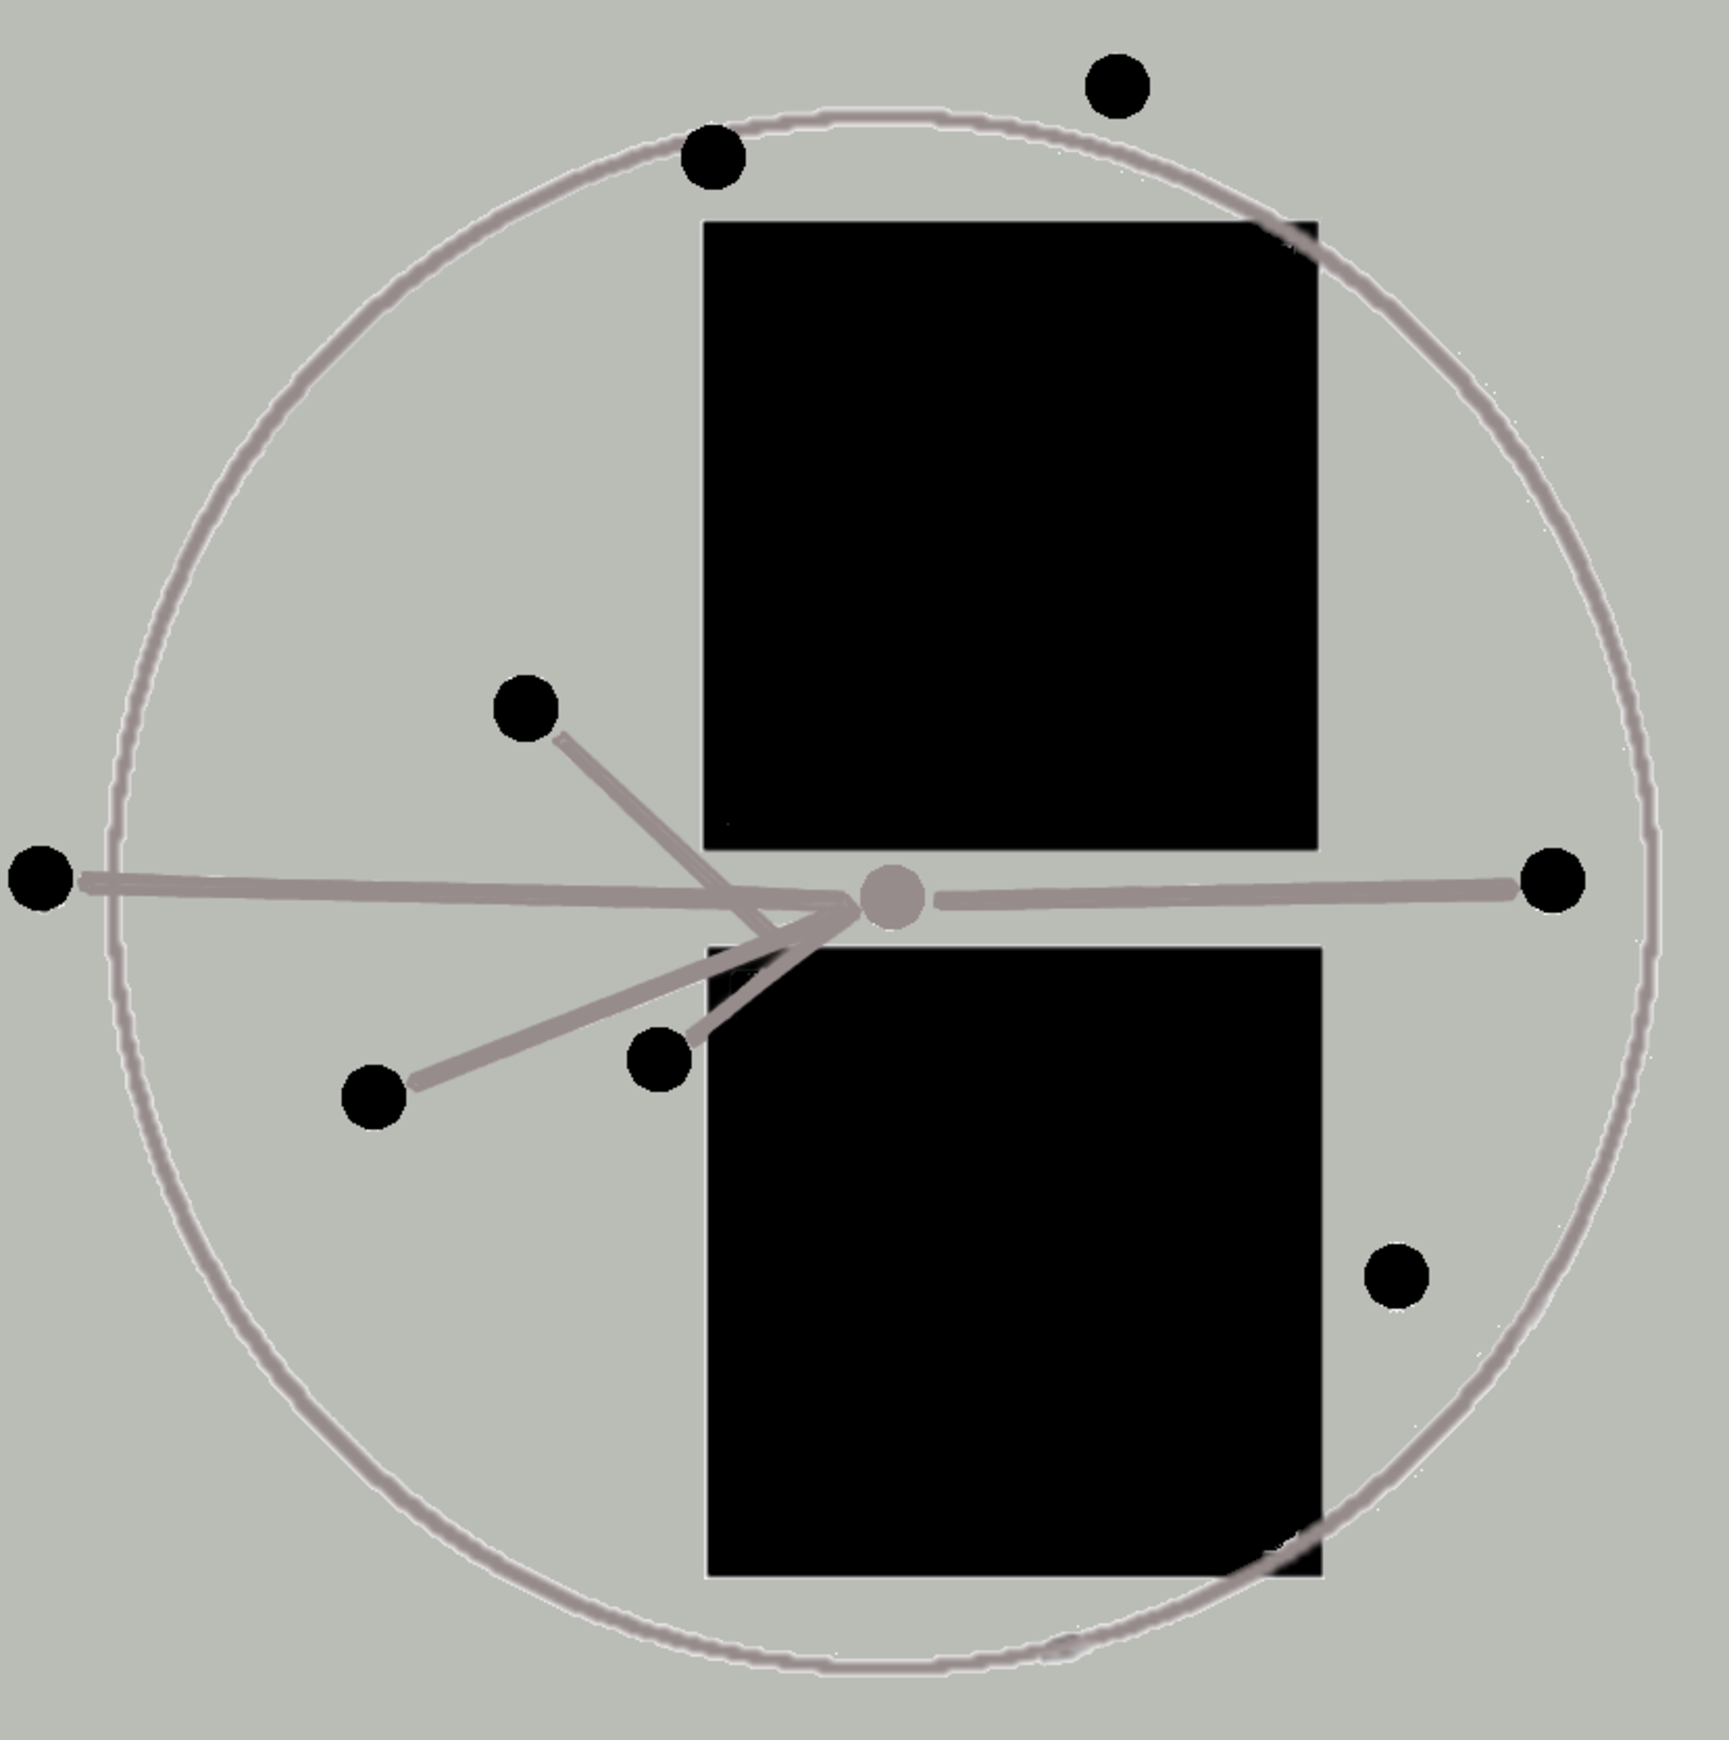
\includegraphics[width=0.3\linewidth]{udgo}
          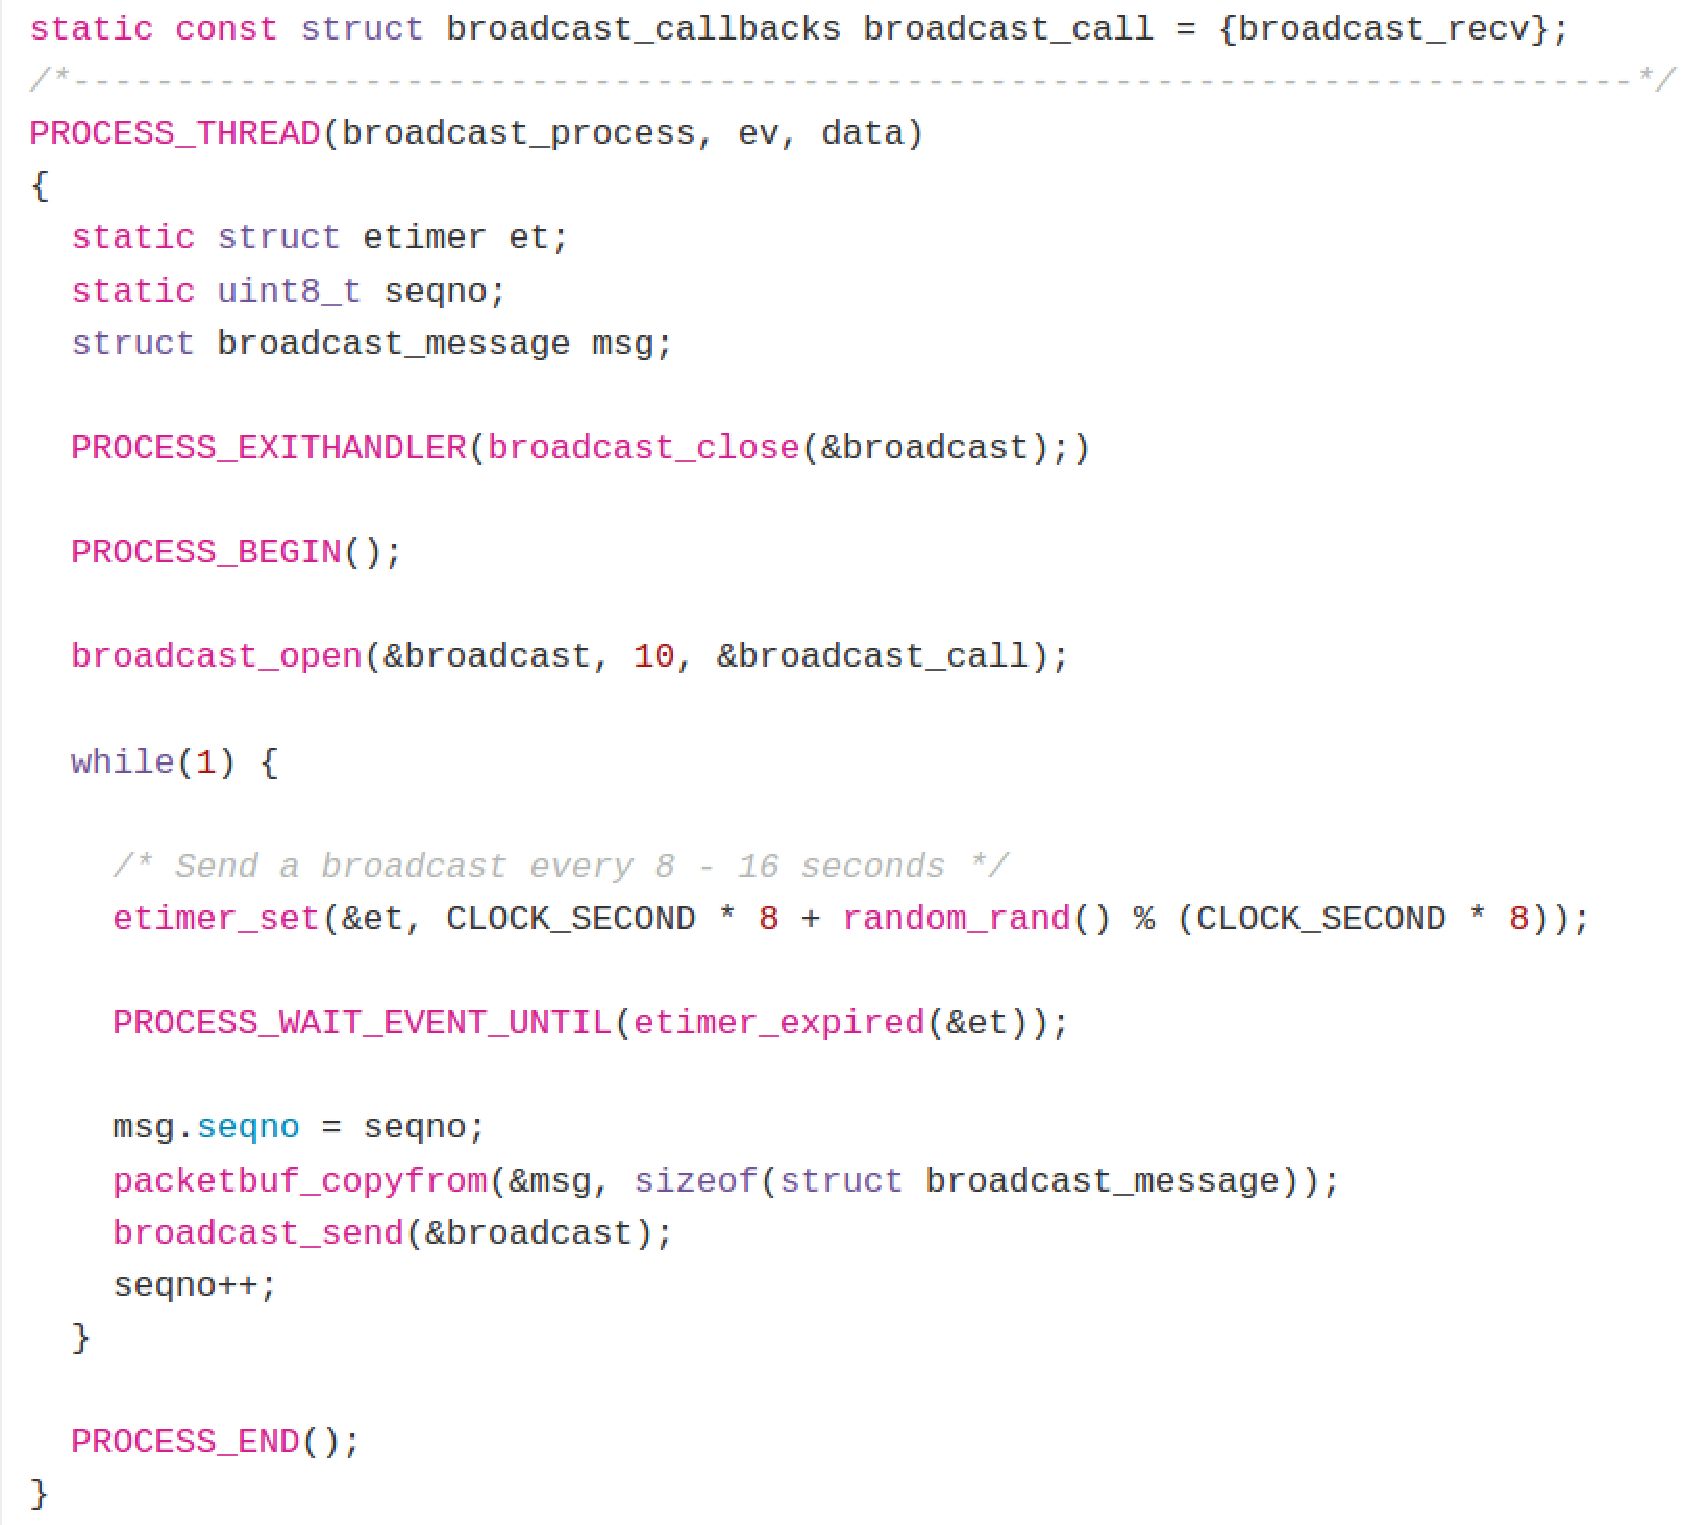
\includegraphics[width=0.3\linewidth]{node-code}
          \begin{itemize}
          \item Experimental: UDGO  {\bf https://github.com/mfer/udgo}
          \item Experimental: simulation in batch-mode
          \item Analytical: model and analytical CTR on obstructed networks
          \end{itemize}          
          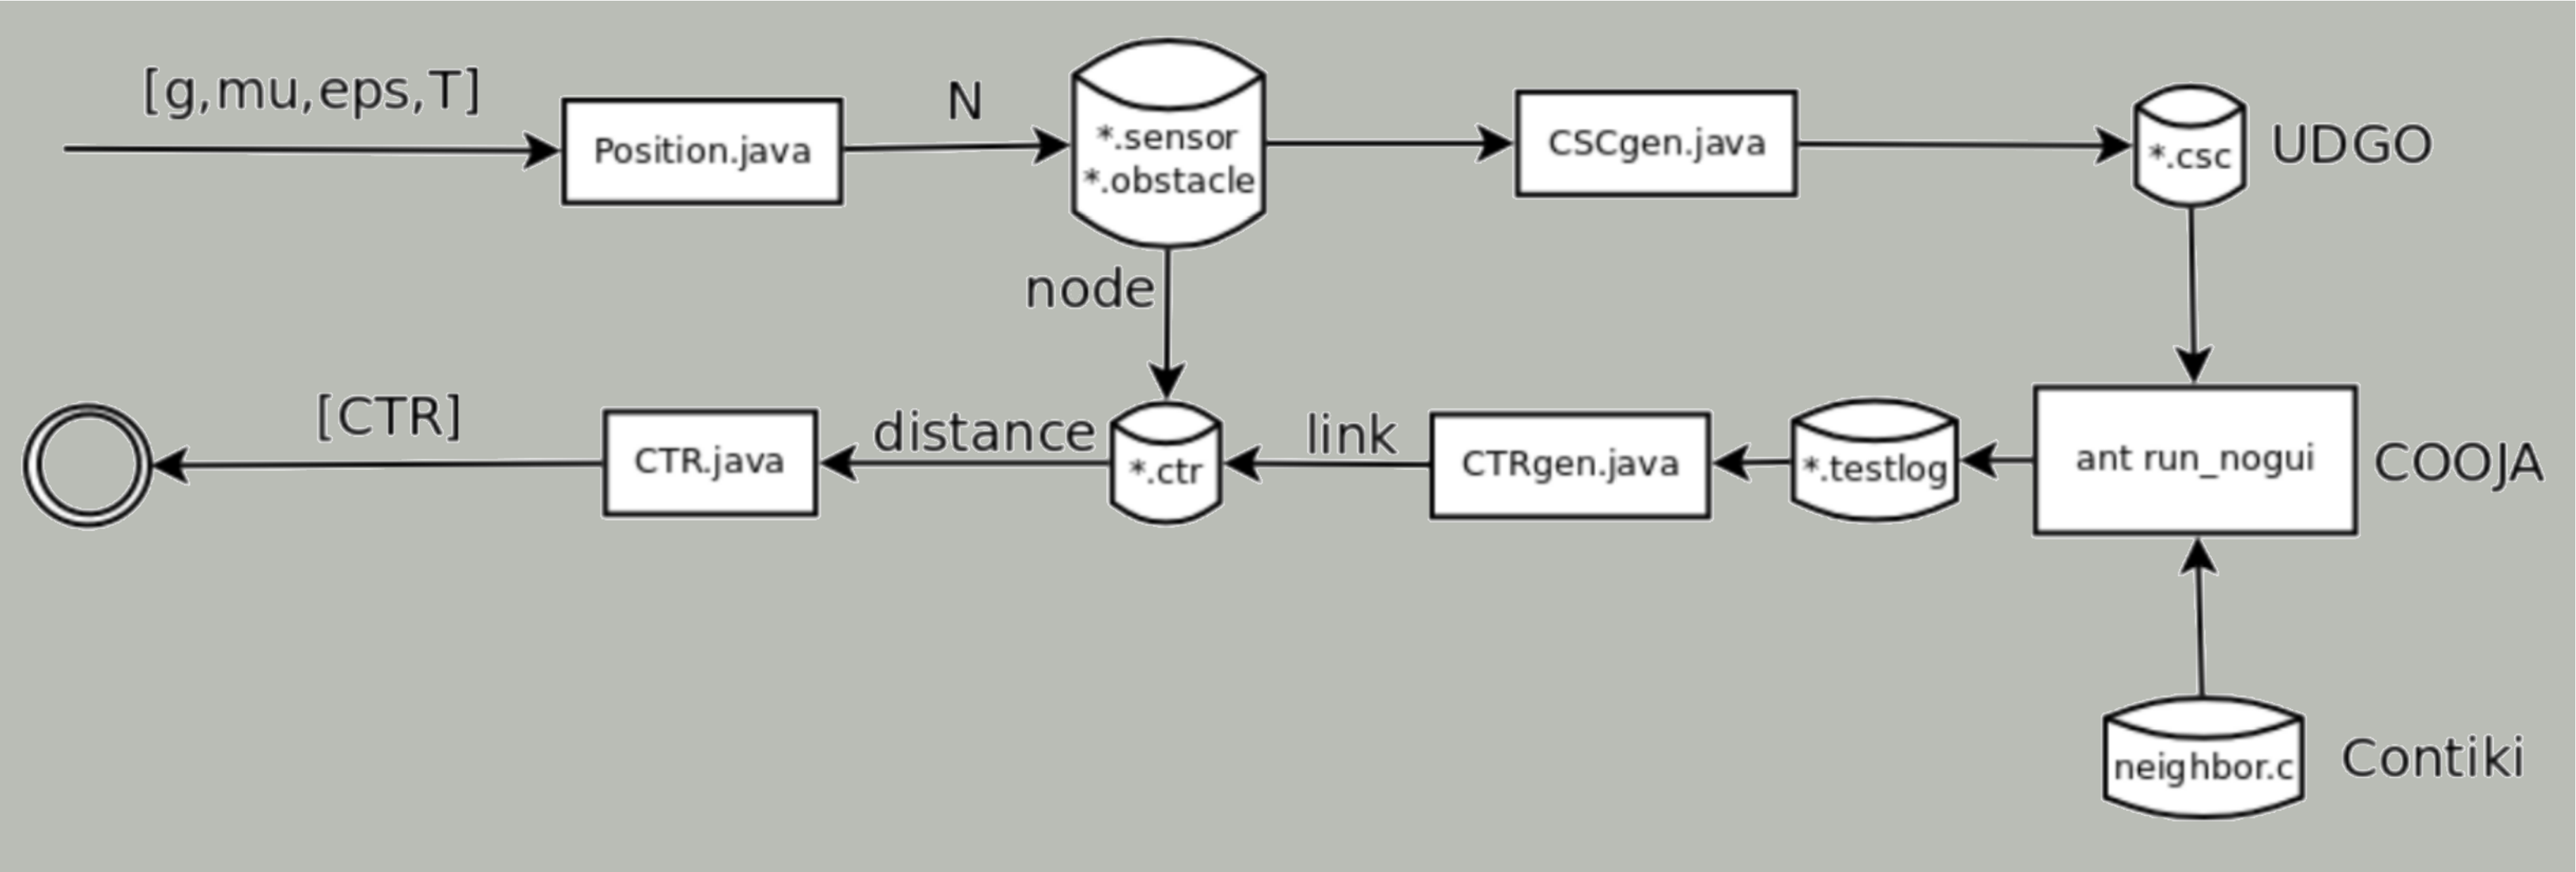
\includegraphics[width=1.0\linewidth]{sim-cycle}
        \end{block}
      \end{column}
      \begin{column}{.48\linewidth}
        \begin{block}{Answers we get}        
          \centering
          We expect discover some insights with the introduced physical medium UDGO that could
          feedback the model. One thing that could happen it will be the experimental CTR be lower
          than the analytical. Due the physical properties introduced with MRM that could make
          visibility increase\newline
        \end{block}  
        \begin{block}{POC2}
          \centering
          On the second part, we performed simulations to study the Critical Transmission Range for Connectivity CTR. Comparing the analytical provided by [Almiron et al. 2013] with the experimental that will be obtained by the authors using the extended COOJA. \newline
          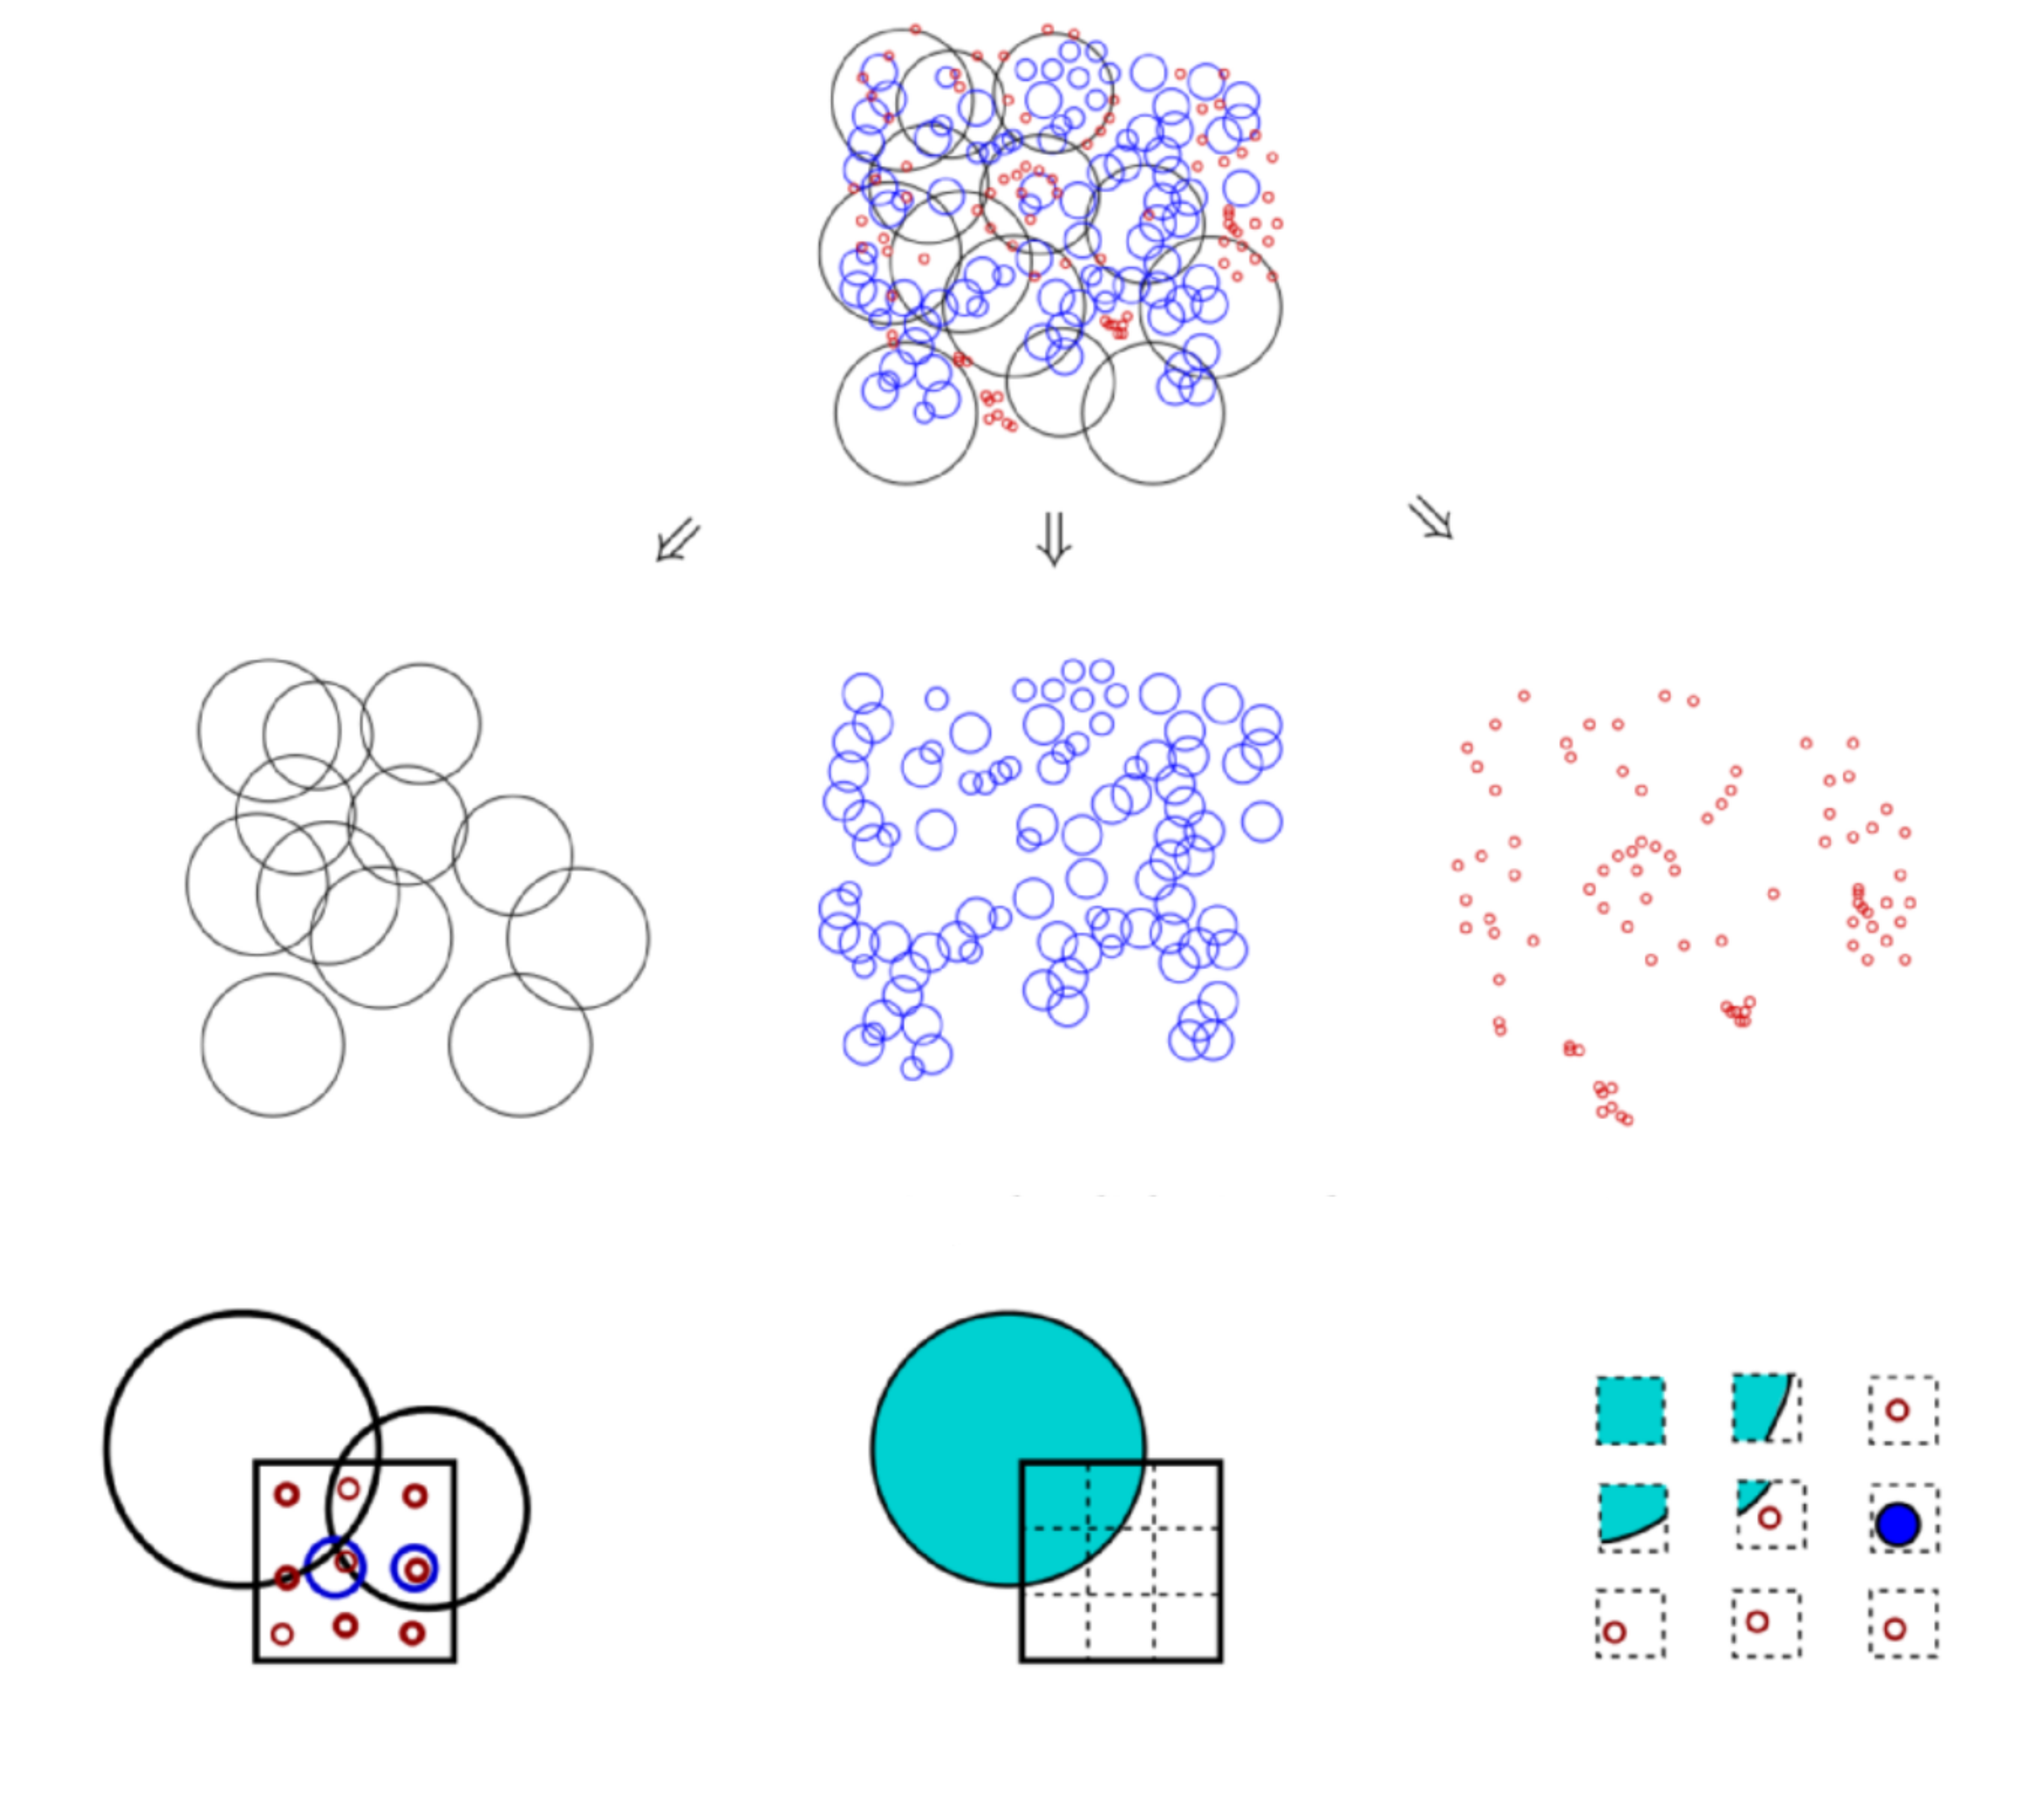
\includegraphics[width=0.75\linewidth]{ptasgig}
          \begin{itemize}
          \item Experimental: client-server
          \item Experimental: simulations
          \item Analytical: PTASGIG {\bf https://github.com/mfer/ptasgig}          
          \end{itemize}  
        \end{block}
      \end{column}
    \end{columns}
    \begin{block}{\footnotesize References}
      \scriptsize
      {\normalsize Almiron et al. 2013} Almiron, M. G., Goussevskaia, O., Loureiro, A. A., 
        and Rolim, J. (2013). Connectivity in obstructed wireless networks: From geometry to 
        percolation. In Proceedings of the ACM, MobiHoc, pages 157-166, New York, NY \newline
      {\normalsize Clark et al. 1990} Clark, B. N., Colbourn, C. J., and Johnson, D. S. (1990). 
        Unit disk graphs. Discrete Mathematics, 86(1 - 3):165 - 177\newline
      {\normalsize Dunkels et al. 2004} Dunkels, A., Gronvall, B., and Voigt, T. (2004). 
        Contiki - a lightweight and flexible operating system for tiny networked sensors. 
        In Local Computer Networks, 2004. 29th Annual IEEE International Conference on, 
        pages 455-462.\newline
      {\normalsize Erlebach et al. 2005} Erlebach, T., Jansen, K., and Seidel, E. (2005). 
        Polynomial-time approximation schemes for geometric intersection graphs. SIAM J. 
        Comput., 34(6):1302-1323. \newline
      {\normalsize Osterlind et al. 2006}  Osterlind, F., Dunkels, A., Eriksson, J., Finne, 
        N., and Voigt, T. (2006). Cross-level sensor network simulation with cooja. In Local 
        Computer Networks, Proceedings 2006 31st IEEE Conference on, pages 641-648.
    \end{block}    
  \end{frame}
\end{document}
